\documentclass[11pt, a4paper]{article}

% Packages
\usepackage[margin=0.5in]{geometry} % Standard 1-inch margins
\usepackage{amsmath, amssymb, amsfonts} % Math packages
\usepackage{graphicx} % For including figures
\usepackage{booktabs} % For professional tables
\usepackage{hyperref} % For hyperlinks
\usepackage[
  backend=biber,
  style=numeric,
  sorting=none,
  maxbibnames=99,
  minbibnames=99,
  maxcitenames=99,
  mincitenames=99
]{biblatex}

\addbibresource{references.bib}
\setlength{\bibhang}{0pt}
\DeclareFieldFormat[article,inbook,incollection,inproceedings,misc,online]{title}{\mkbibemph{#1}}
\usepackage{xcolor} % For colored text (e.g., TODOs)
\usepackage{enumitem} % For list formatting
\usepackage{caption}
\usepackage{subcaption}
\usepackage{indentfirst}
\usepackage{longtable}
\usepackage{float}

\hypersetup{
  colorlinks=true,
  linkcolor=blue,
  filecolor=magenta,
  urlcolor=cyan,
  citecolor=blue,
}

\title{COMP9417 Project: Feature learning kernel machines for tabular data \\ \large [One Night Miracle]}

\author{
  Chih-Yueh Liu \\
  z5631242 \\
  UNSW Sydney \\
  \texttt{z5631242@ad.unsw.edu.au}
  \and
  Isaac Dwadattusyah Haikal Azziz \\
  z5640942 \\
  UNSW Sydney \\
  \texttt{z5640942@ad.unsw.edu.au}
  \and
  Enjia Wu \\
  z5456801 \\
  UNSW Sydney \\
  \texttt{z5456801@ad.unsw.edu.au}
  \and
  Jialong (Alan) Wang \\
  z5696241 \\
  UNSW Sydney \\
  \texttt{alanwing1997@gmail.com}
  \and
  Chalat Phumphiraratthaya \\
  z5623543 \\
  UNSW Sydney \\
  \texttt{z5623543@ad.unsw.edu.au}
}
\date{\today}

\begin{document}

\maketitle
\thispagestyle{empty} % No page number on title page

\vspace{2cm}
\newpage
\begin{abstract}
  This project explores the application of feature learning kernel machines for tabular data. We implement the newly published feature learning kernel machine, i.e. xRFM~\cite{ref1}, according to the paper and evaluate its performance with traditional kernel machines and deep learning models on a suite of benchmark datasets. Specifically, we compare xRFM against 3 baselines: Random Forest, XGBoost, and TabPFN. We evaluate performance using RMSE for regression tasks and Accuracy/AUC-ROC for classification tasks, as well as training and inference time. Additionally, we analyze the interpretability of xRFM by comparing its feature importance scores with those from traditional methods. Finally, we assess the scalability of xRFM on larger datasets by plotting performance and training time against the number of samples. Our experiments demonstrate that feature learning kernel machines can achieve competitive performance on tabular data, and that they are particularly effective for datasets with complex relationships between features and target variables.
\end{abstract}

\section{Introduction}
Tabular data remains one of the most important data formats in practical machine learning. Many high-value prediction problems, such as risk assessment and health-related prediction, are naturally represented as tables, where rows are observations and columns are structured variables. Yet supervised learning on tabular data has progressed more slowly than in vision or language, and strong tree-based methods such as GBDTs remain difficult to displace in practice~\cite{ref1}.

A key reason is that tabular data has a different structure from images and text. In images, nearby pixels have local spatial relationships~\cite{ref2}, and in language, tokens derive meaning from sequence context~\cite{ref3}. By contrast, tabular features often have standalone semantic meaning, and different parts of the input space may depend on different predictive variables~\cite{ref1}. This makes it hard for a single global model to capture all relevant patterns well, especially on heterogeneous datasets~\cite{ref1}.

xRFM is designed to address this gap by combining a feature-learning kernel model with an adaptive binary tree~\cite{ref1}. At each internal node, it uses the Average Gradient Outer Product (AGOP) to choose a split direction, and at each leaf it fits a local Recursive Feature Machine~\cite{ref1,ref4}. This is interesting for two reasons: it allows feature relevance to vary across regions of the data space, and it improves scalability by replacing one large global kernel problem with a hierarchy of smaller local ones~\cite{ref1}.

In this project, we evaluate xRFM on five tabular datasets---Abalone, Diamonds, Superconductor, Obesity Level, and Sleep Health---covering three regression tasks, two classification tasks, mixed-type features, a high-dimensional dataset, and large-sample settings. We compare it with XGBoost, Random Forest, and TabPFN, and also study AGOP-based interpretability and learning-curve behaviour. Overall, our results show that xRFM is a competitive and interpretable method: it performs strongly on several tasks and is often close to the best baseline, but it does not consistently outperform TabPFN or XGBoost across all datasets, especially on the more challenging large-scale classification setting.

\section{Methodology}
\subsection{Average Gradient Outer Product}

A core object in xRFM is the \textbf{Average Gradient Outer Product (AGOP)}. For a trained scalar-valued predictor \(f : \mathbb{R}^{d} \rightarrow \mathbb{R}\) and a dataset \(S = \{x^{(1)}, \ldots, x^{(n)}\} \subset \mathbb{R}^{d}\), it is defined as
\[
  AGOP(f,S) = \frac{1}{n}\sum_{i=1}^{n} \nabla f\!\left(x^{(i)}\right)\nabla f\!\left(x^{(i)}\right)^{\top}.
\]

It measures how sensitive the fitted predictor is, on average, to small input perturbations. Because each term is an outer product of a gradient vector with itself, the AGOP is symmetric and positive semidefinite. The \((j,k)\)-th entry measures how sensitivities along features \(j\) and \(k\) co-vary, while
\[
  AGOP_{jj}
  =
  \frac{1}{n}\sum_{i=1}^{n}
  \left(
    \frac{\partial f\!\left(x^{(i)}\right)}{\partial x_j}
  \right)^2
\]
is the average squared partial derivative for feature \(j\). A large diagonal entry means the predictor changes strongly when that feature changes, whereas a small entry indicates relative insensitivity to that coordinate.

AGOP supports two complementary interpretability views. Its diagonal gives coordinate-wise feature importance, while its leading eigenvectors identify directions in input space along which the predictor varies most. For any unit vector \(v\),
\[
  v^{\top} AGOP(f,S)\, v
  =
  \frac{1}{n}\sum_{i=1}^{n}
  \left(
    \nabla f\!\left(x^{(i)}\right)^{\top} v
  \right)^2,
\]
so the top eigenvector gives the direction with the largest average squared directional derivative. Thus, the diagonal captures axis-aligned importance, whereas the eigendecomposition captures joint feature effects. This matters in tabular learning because predictive structure may depend not only on single variables but also on interactions among them.

Compared with simpler feature-analysis methods, \textbf{AGOP} is supervised and model-based. \textbf{PCA} is unsupervised and identifies directions of large input variance whether or not they are predictive. \textbf{Mutual information} is usually applied one feature at a time and therefore does not directly recover joint predictive directions. \textbf{Permutation importance} measures performance loss after feature shuffling, so it is useful as a post hoc score but does not provide the same geometric description of the learned predictor. By contrast, AGOP summarises both single-feature relevance and multi-feature predictive structure in a single matrix.

\subsection{xRFM Training Pipeline}

xRFM combines a feature-learning kernel model with an adaptive binary tree. It is motivated by two limitations of standard kernel methods: the kernel is fixed in advance and may not align with the most predictive structure, and exact training requires solving a large kernel system. xRFM addresses the first problem through AGOP-based feature learning and the second through recursive partitioning.

At each leaf, xRFM uses a modified Recursive Feature Machine (RFM), which alternates between fitting a kernel predictor and updating a feature matrix using the AGOP of the fitted model. For tabular data, xRFM extends this idea by searching over a broader kernel family, allowing either the full AGOP or only its diagonal, handling categorical variables explicitly, and selecting bandwidth locally within each leaf. These choices are useful because tabular columns often have distinct semantic meaning and different regions of the feature space may follow different predictive patterns.

The tree is built recursively. At each node, xRFM fits a temporary split model, computes its AGOP, and takes the leading eigenvector as the split direction. The data are then divided by the median projection onto that direction, which keeps the tree approximately balanced. Splitting continues until each leaf contains at most \(C\) samples, after which a full leaf RFM is trained on that subset. For a new point \(x^{*}\), inference routes it from the root to a terminal leaf using the stored split rules, and the leaf-specific RFM produces the final prediction. By replacing one large global kernel problem with a hierarchy of smaller local ones, xRFM improves scalability while remaining locally adaptive; in the xRFM framework, training is approximately \(O(n \log n)\) and inference is \(O(\log n)\).

\subsection{Experimental Setup}

We compared \textbf{xRFM}, \textbf{XGBoost}, \textbf{Random Forest}, and \textbf{TabPFN} on five tabular datasets: \textbf{Abalone}, \textbf{Diamonds}, \textbf{Superconductor}, \textbf{Obesity Level}, and \textbf{Sleep Health}. This selection covers both regression and classification, including at least one large-$n$ dataset, one high-dimensional dataset, and one dataset with mixed numerical and categorical features. All experiments used a fixed random seed of 9417 for reproducibility. We used \textbf{TabPFN v2.6} in our experiments, as it offers a strong and up-to-date baseline for tabular learning.

Each dataset was preprocessed into fixed training and test sets using a held-out 20\% test split. For classification datasets, stratified splitting was used to preserve class proportions. We did not store a separate validation file; instead, hyperparameters were selected by 5-fold cross-validation on the training split only, and final results were reported on the untouched test split. xRFM, XGBoost, and Random Forest were tuned with 100-trial searches, using \texttt{KFold} for regression and \texttt{StratifiedKFold} for classification. The final model for each dataset was the configuration with the best validation performance, then refit on the full training split.

Preprocessing was model-specific. For xRFM, XGBoost, and Random Forest, categorical and binary features were one-hot encoded before fitting. The main difference between these models was the treatment of numerical variables: xRFM standardised them, whereas XGBoost and Random Forest used them as passthrough (unscaled) inputs. TabPFN used the processed features directly, with no additional scaling or encoding applied at the model stage.

We report \textbf{RMSE} for regression because it directly measures the magnitude of continuous prediction error and penalises larger errors more heavily. For classification, we report both \textbf{Accuracy} and \textbf{AUC-ROC}: Accuracy measures overall correctness, while AUC-ROC evaluates class separability across decision thresholds; for multiclass tasks, AUC-ROC was computed using a one-vs-rest formulation. We also record training time and inference time per sample to compare computational efficiency across methods. Beyond the main benchmark, we performed an interpretability comparison on Abalone using AGOP, PCA, mutual information, and permutation importance, and a learning-curve experiment on a large dataset to examine how performance and runtime change with sample size.

The final hyperparameter configuration selected for each model on each dataset is summarised in (Appendix~\ref*{app:final-configs}; Tables~\ref{tab:xrfm-config}--\ref{tab:tabpfn-config}).

\section{Results}
\subsection{Overall Performance}

\begin{table}[H]
  \centering
  \caption{Test performance across datasets. For regression tasks we report RMSE; for classification tasks we report Accuracy and AUC-ROC.}
  \scriptsize
  \resizebox{\textwidth}{!}{
    \begin{tabular}{lcccc}
      \toprule
      \textbf{Dataset} & \textbf{xRFM} & \textbf{XGBoost} & \textbf{Random Forest} & \textbf{TabPFN} \\
      \midrule
      Abalone (RMSE) & 2.1013 & 2.1737 & 2.1891 & 2.0549 \\
      Diamonds (RMSE) & 520.0493 & 562.1491 & 833.2694 & 519.3203 \\
      Superconductor (RMSE) & 9.8139 & 9.4001 & 10.7205 & 9.1863 \\
      Obesity Level (Acc./AUC) & 0.9835 / 0.9997 & 0.9669 / 0.9990 & 0.9433 / 0.9926 & 0.9929 / 1.0000 \\
      Sleep Health (Acc./AUC) & 0.8905 / 0.9756 & 0.9465 / 0.9909 & 0.8458 / 0.9682 & 0.9435 / 0.9933 \\
      \bottomrule
    \end{tabular}
  }
  \label{tab:overall_performance}
\end{table}

\begin{table}[H]
  \centering
  \caption{Compute cost across datasets: training time and inference time per sample.}
  \scriptsize
  \resizebox{\textwidth}{!}{%
    \begin{tabular}{lcccccccc}
      \toprule
      \textbf{Dataset} &
      \textbf{xRFM Fit (s)} & \textbf{xRFM Inf./Sample (s)} &
      \textbf{XGB Fit (s)} & \textbf{XGB Inf./Sample (s)} &
      \textbf{RF Fit (s)} & \textbf{RF Inf./Sample (s)} &
      \textbf{TabPFN Fit (s)} & \textbf{TabPFN Inf./Sample (s)} \\
      \midrule
      Abalone & 0.4593 & $1.01 \times 10^{-5}$ & 0.1895 & $2.69 \times 10^{-6}$ & 0.0593 & $4.43 \times 10^{-5}$ & 0.9748 & $2.66 \times 10^{-3}$ \\
      Diamonds & 80.3824 & $1.10 \times 10^{-4}$ & 0.4962 & $6.95 \times 10^{-7}$ & 0.1017 & $2.65 \times 10^{-6}$ & 3.6773 & $6.97 \times 10^{-2}$ \\
      Superconductor & 12.8962 & $5.03 \times 10^{-5}$ & 2.0742 & $2.63 \times 10^{-6}$ & 0.2184 & $6.45 \times 10^{-6}$ & 6.4547 & $7.93 \times 10^{-2}$ \\
      Obesity Level & 0.1568 & $7.32 \times 10^{-6}$ & 0.6880 & $6.67 \times 10^{-5}$ & 0.1095 & $6.01 \times 10^{-5}$ & 0.2680 & $1.88 \times 10^{-3}$ \\
      Sleep Health & 11.6116 & $4.97 \times 10^{-5}$ & 1.4002 & $4.75 \times 10^{-6}$ & 0.1477 & $6.56 \times 10^{-6}$ & 1.7053 & $1.06 \times 10^{-2}$ \\
      \bottomrule
    \end{tabular}%
  }
  \label{tab:compute_cost}
\end{table}

Overall, XGBoost and TabPFN deliver strong predictive performance across both regression and classification tasks (Table~\ref{tab:overall_performance}). xRFM is competitive on several datasets, but its training time can be substantially higher on larger problems (e.g., Diamonds) (Table~\ref{tab:compute_cost}). TabPFN remains accurate but has noticeably higher inference time per sample, while tree-based baselines tend to offer a favorable accuracy--efficiency trade-off.

For additional per-class diagnostics on the two classification datasets, we include confusion matrices (Appendix~B; Figures~\ref{fig:cm-obesity}--\ref{fig:cm-sleep-health}), ROC curves (Appendix~C; Figures~\ref{fig:roc-obesity} and~\ref{fig:roc-sleep}), and detailed classification reports (Appendix~D; Tables~\ref{tab:obesity_classification_report} and~\ref{tab:sleep_health_classification_report}).

\subsection{Interpretability Comparison}
Following the project specification, we perform an interpretability comparison on dataset \textbf{Abalone} by extracting the AGOP diagonal from a trained xRFM model (using the leaf AGOP matrix) and comparing it to three classical feature importance baselines computed on the same processed features: (i) PCA variance-weighted loadings, (ii) mutual information between features and the target, and (iii) permutation importance measured via change in test RMSE. Figure~\ref{fig:interpretability_importance_bar} shows the normalised importance magnitudes, while Figure~\ref{fig:interpretability_bump_chart} visualises how the top-ranked features change across methods.

Across all methods, weight-related features (e.g., \texttt{whole\_weight}, \texttt{shucked\_weight}, and \texttt{shell\_weight}) are consistently identified as most informative, whereas the one-hot \texttt{sex\_*} variables remain low-importance. The methods diverge in the ordering of the mid-ranked geometric features (\texttt{length}, \texttt{diameter}, \texttt{height}) and in how strongly they emphasise \texttt{shell\_weight}: mutual information ranks it highest, while AGOP and permutation importance place it slightly lower. In conclusion, the agreement on the dominant features supports the use of the AGOP diagonal as a meaningful, model-specific importance measure, with differences reflecting that each baseline captures a different notion of ``importance'' (variance structure, marginal dependence, or predictive sensitivity).

\begin{figure}[H]
  \centering
  \begin{subfigure}[b]{0.49\textwidth}
    \centering
    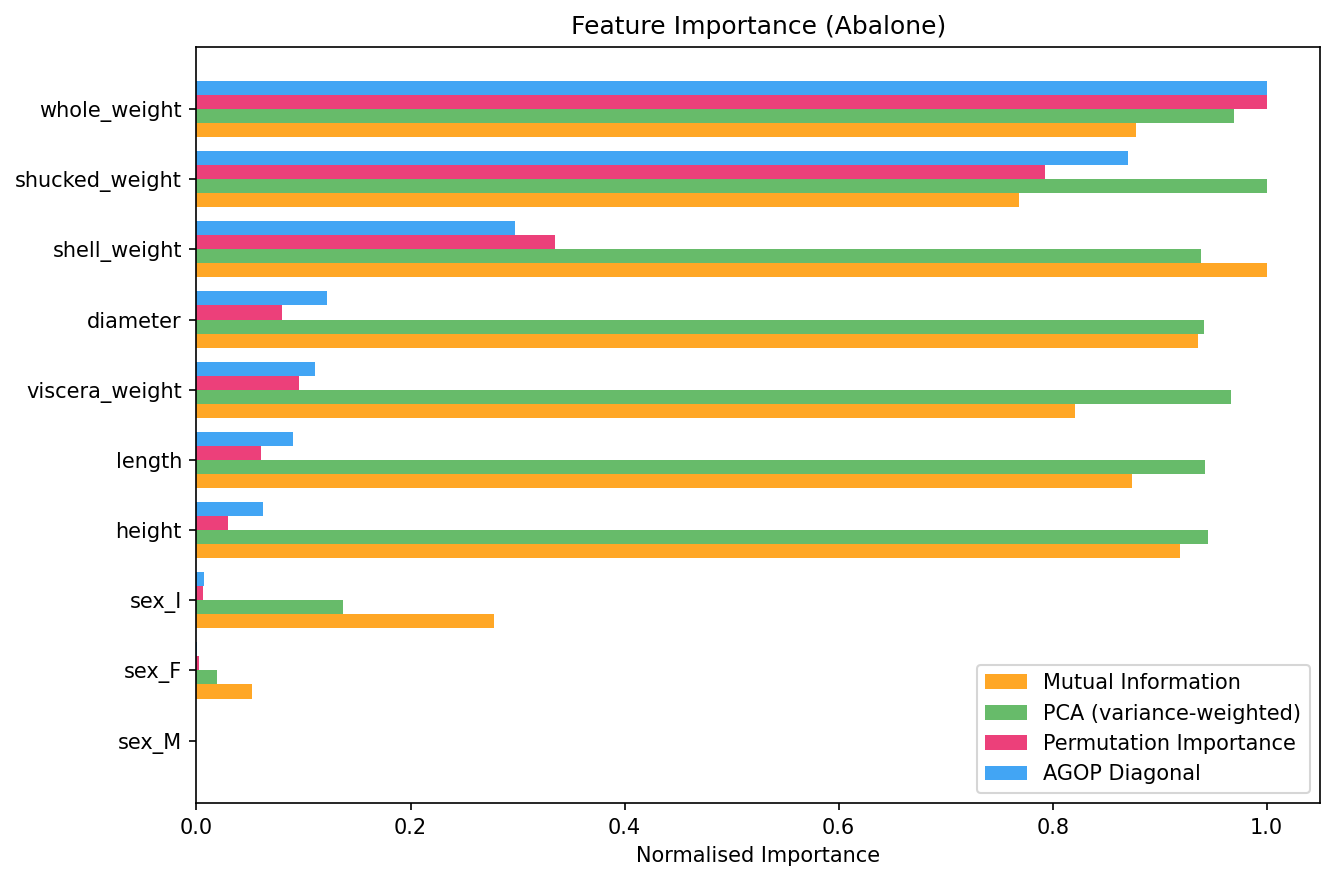
\includegraphics[width=\textwidth]{../results/03_interpretability/importance_bar.png}
    \caption{Normalised feature importance scores}
    \label{fig:interpretability_importance_bar}
  \end{subfigure}
  \hfill
  \begin{subfigure}[b]{0.49\textwidth}
    \centering
    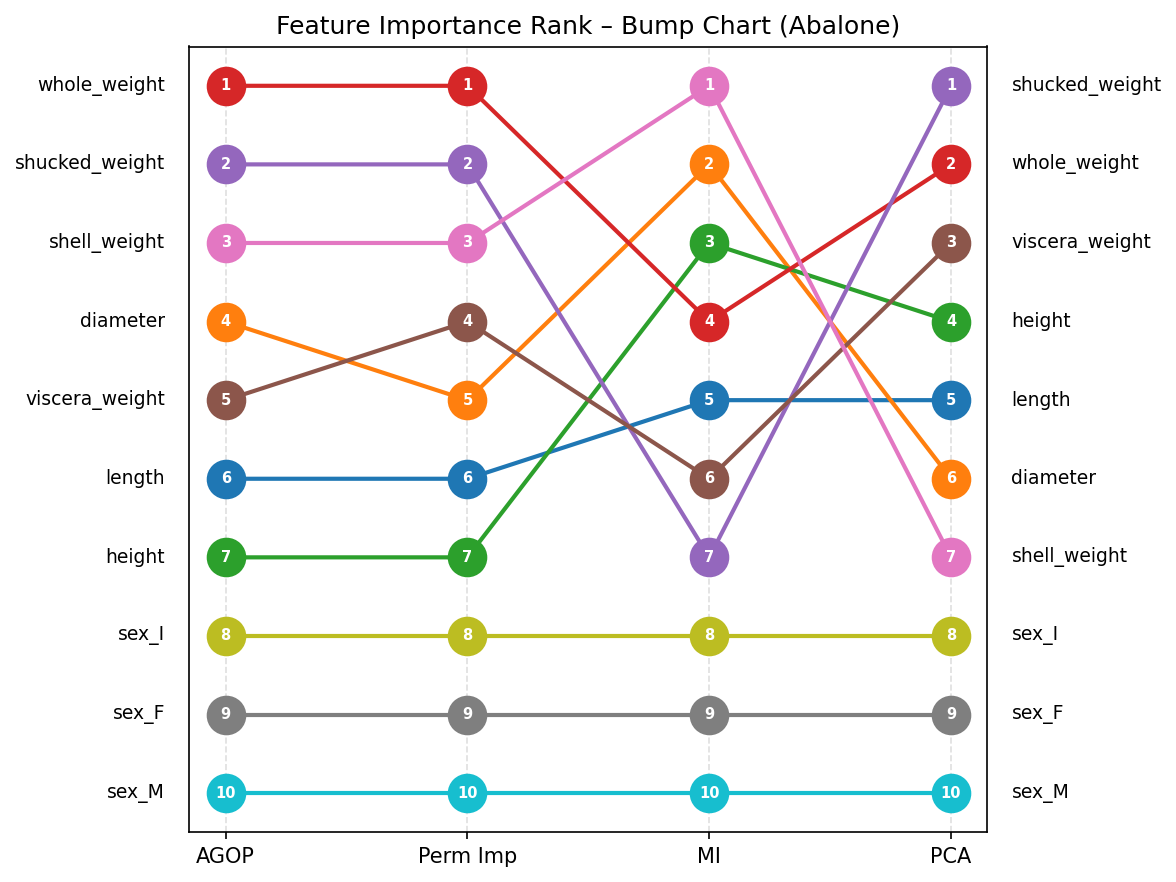
\includegraphics[width=\textwidth]{../results/03_interpretability/bump_chart.png}
    \caption{Rank comparison across methods}
    \label{fig:interpretability_bump_chart}
  \end{subfigure}
  \caption{Interpretability comparison on the Abalone dataset. We compare xRFM's AGOP-diagonal feature importances against PCA (variance-weighted loadings), mutual information, and permutation importance.}
  \label{fig:interpretability}
\end{figure}

\subsection{Scalability Analysis}
% On one large dataset (n > 10,000), subsample the training set at several sizes and plot test performance and training time versus n for all models.
\begin{figure}[H]
  \centering
  \begin{subfigure}[b]{0.32\textwidth}
    \centering
    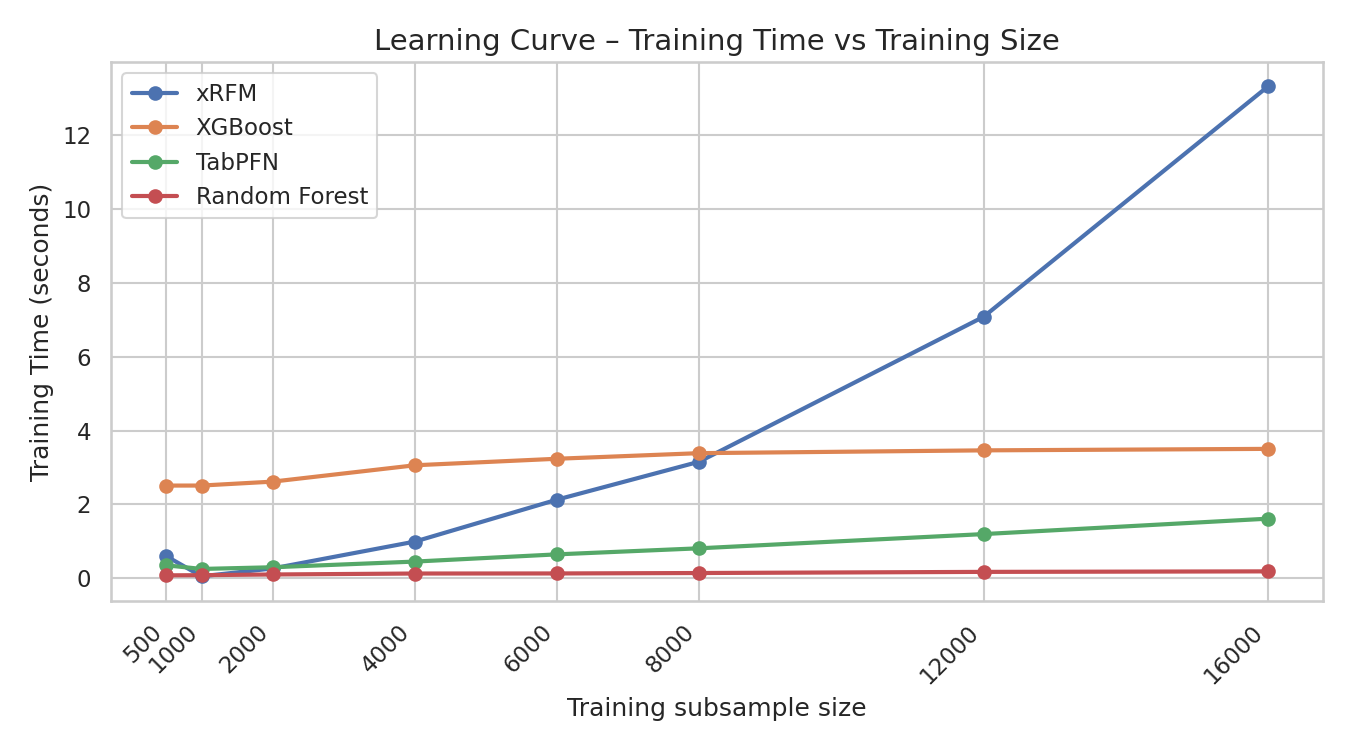
\includegraphics[width=\textwidth]{../results/04_learning_curve/learning_curve_sleep_health_fit_time.png}
    \caption{Training time}
    \label{fig:scalability_sleep_health_fit_time}
  \end{subfigure}
  \hfill
  \begin{subfigure}[b]{0.32\textwidth}
    \centering
    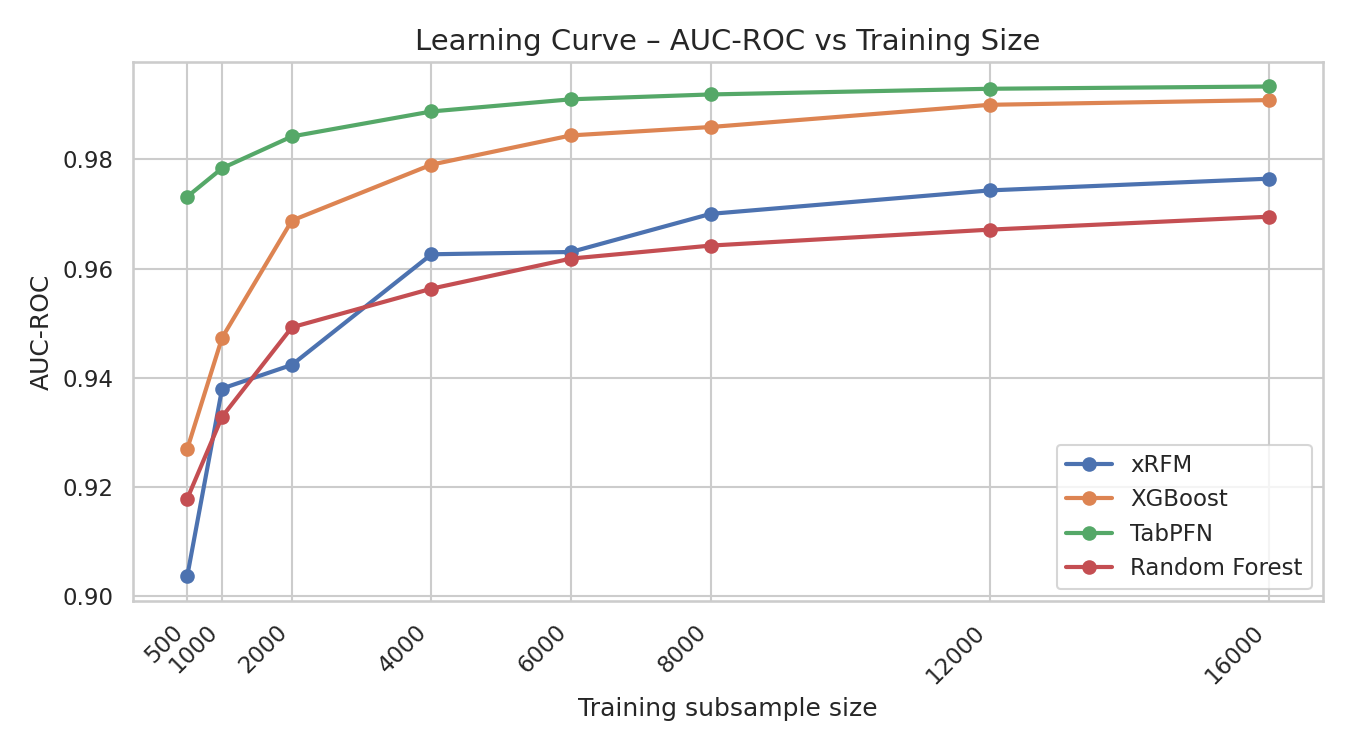
\includegraphics[width=\textwidth]{../results/04_learning_curve/learning_curve_sleep_health_auc_roc.png}
    \caption{AUC-ROC}
    \label{fig:scalability_sleep_health_auc_roc}
  \end{subfigure}
  \hfill
  \begin{subfigure}[b]{0.32\textwidth}
    \centering
    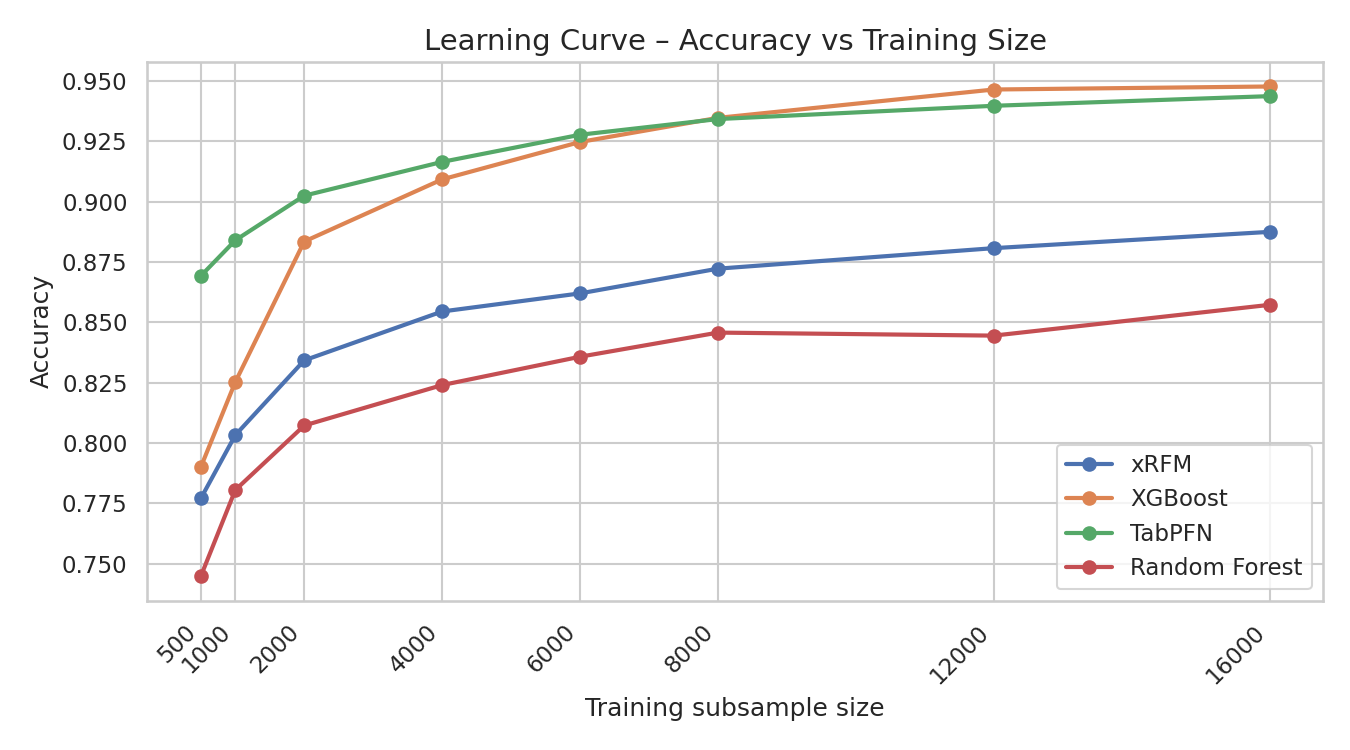
\includegraphics[width=\textwidth]{../results/04_learning_curve/learning_curve_sleep_health_accuracy.png}
    \caption{Accuracy}
    \label{fig:scalability_sleep_health_accuracy}
  \end{subfigure}
  \caption{Scalability analysis on the Sleep Health dataset (classification task; target: \texttt{sleep\_disorder\_risk}). We plot training time and test performance against the number of training samples $n$ for all models.}
  \label{fig:scalability}
\end{figure}

We evaluate scalability on the Sleep Health dataset, a multi-class classification task that predicts the \texttt{sleep\_disorder\_risk} label from mixed numerical and categorical features. As the training subsample size $n$ increases, we observe consistent improvements in predictive performance for all models in terms of both AUC-ROC and Accuracy, with gains diminishing as curves begin to saturate at larger $n$. In contrast, training time generally increases with $n$: xRFM exhibits the steepest growth in total training time as $n$ becomes large, while tree-based baselines (Random Forest and XGBoost) remain comparatively stable in this range, and TabPFN stays fast across all subsample sizes. Overall, these results highlight the expected trade-off between improved generalization from more data and the computational cost of training, and show that different model families scale quite differently on the same large tabular classification dataset.


\section{Discussion}
Overall, our results match part of what we would expect from the idea behind xRFM. xRFM is built for tabular data: it uses a tree to split the dataset into simpler local regions, and then learns flexible, nonlinear patterns within each region instead of relying on a fixed feature map. After preprocessing, both continuous variables and one-hot encoded categorical variables become numeric inputs, so in principle xRFM can handle a wide mix of feature types and tasks. This makes it reasonable that xRFM is often competitive with strong baselines, especially when the target depends on nonlinear interactions and there is enough data for the AGOP-based split directions to be learned reliably. At the same time, our experiments do not show xRFM as a clear overall winner. TabPFN is the most accurate model across our suite, Random Forest is usually the weakest, and xRFM and XGBoost trade places depending on the dataset. In short, xRFM performs best when it can make use of meaningful nonlinear structure in the data, but it can fall short in harder settings where its splitting and feature-learning pipeline is less stable, so its advantage over XGBoost appears real on some datasets but not consistent enough to be called a universal improvement.

The feature-importance comparison mostly supports the interpretation of AGOP given in the Methodology. On Abalone, the AGOP diagonal identifies the same broad group of important features as the other methods: weight-related variables such as \texttt{whole\_weight}, \texttt{shucked\_weight}, and \texttt{shell\_weight} are consistently ranked near the top, while the one-hot \texttt{sex\_*} features remain near the bottom. This agrees with the idea that the AGOP diagonal measures how sensitive the trained xRFM model is to each input coordinate. It is also useful that AGOP is especially close to permutation importance for the top two features, since permutation importance directly measures how much the model relies on a feature for prediction. The main differences appear in the middle of the ranking: for example, mutual information gives very high rank to \texttt{shell\_weight} and \texttt{diameter}, while PCA ranks some geometric features higher because it is driven by input variance rather than prediction. This was not a major contradiction, but it was a useful reminder that each method defines ``importance'' differently. Overall, the comparison suggests that AGOP gives a meaningful model-specific explanation of xRFM, while the disagreements with PCA and MI show that it is not merely recovering generic variance or marginal dependence patterns.

In our experiments, xRFM underperforms XGBoost most clearly on Sleep Health and Superconductor. For Sleep Health, XGBoost achieves 0.9465 Accuracy and 0.9909 AUC-ROC, compared to 0.8905 Accuracy and 0.9756 AUC-ROC for xRFM; for Superconductor, XGBoost attains a lower RMSE (9.4001 vs. 9.8139). A possible hypothesis according to xRFM’s design is that its AGOP-driven splitting becomes less reliable as the effective feature dimension grows after preprocessing, since each leaf relies on estimating a $d\times d$ AGOP matrix and extracting a leading direction from it. When $d$ is large---especially with sparse one-hot expansions (as in Sleep Health) or strong multicollinearity and redundancy among continuous descriptors (as in Superconductor)---the local feature geometry may be harder to estimate accurately, causing split directions to be noisier and downstream leaf RFMs to generalize less well. This hypothesis is consistent with the fact that the two datasets where xRFM loses most are also among the highest-dimensional settings in our suite, whereas XGBoost can more easily ignore weak or redundant dimensions through axis-aligned tree splits. That said, this evidence is correlational: confirming the mechanism would require controlled studies that vary $d$ and sparsity (e.g., ablations on one-hot cardinality or feature selection) to test whether performance degrades systematically for AGOP-based splitting in high-dimensional tabular regimes.

If we had more time, we would strengthen the empirical conclusions by broadening both the experimental scope and the analysis tools. On the scalability and performance side, we would add more datasets whose characteristics stress the regimes where xRFM may be less robust---such as higher effective dimensionality, strongly correlated continuous features, and sparse one-hot categorical expansions---to test whether the observed weaknesses are systematic rather than dataset-specific. We would also allocate a larger tuning budget to xRFM, whose computational cost limited the number of configurations explored compared to XGBoost, and search more extensively over kernel choices and bandwidth, regularization, leaf size, the use of full versus diagonal AGOP, and the number of RFM iterations; in addition, we would compare different tuning objectives (e.g., F1 and AUC-ROC instead of accuracy for potentially imbalanced classification tasks, and alternative regression losses beyond RMSE) to better match evaluation goals. Finally, for interpretability, we would extend the comparison beyond PCA/MI/permutation by including methods such as SHAP and by contrasting against feature importance derived from strong tree baselines (Random Forest/XGBoost), helping to clarify whether AGOP provides a genuinely distinct, model-specific perspective or largely agrees with established explanations.


\section{Conclusion}
We evaluated xRFM on five tabular datasets and compared it with XGBoost, Random Forest, and TabPFN across both regression and classification tasks. Overall, xRFM is competitive and offers a useful AGOP-based interpretability story, but it does not consistently outperform the strongest baselines.

Our interpretability results on Abalone broadly agree with standard importance methods, while providing a model-specific view via feature sensitivities. On the efficiency side, the learning-curve experiment highlights a practical trade-off: xRFM can be much slower to train on larger problems and may fall behind XGBoost/TabPFN in some settings. Taken together, xRFM is best viewed as a strong, interpretable option for tabular learning rather than a universal replacement.

\newpage
\printbibliography[title={References}]

\newpage
\appendix
\section*{Appendix}
\section{Final model configurations used in the benchmark}
\label{app:final-configs}

Tables~\ref{tab:xrfm-config}, \ref{tab:xgb-config}, \ref{tab:rf-config}, and \ref{tab:tabpfn-config} summarise the final hyperparameter configurations selected for each model on each dataset. Only model settings are reported here; predictive performance is presented separately in the Results section.

\subsection{xRFM}
\label{tab:xrfm-config}

\begin{table}[h]
  \centering
  \small
  \setlength{\tabcolsep}{5pt}
  \caption{Final xRFM configurations across datasets.}
  \label{tab:xrfm-config}
  \begin{tabular}{lccccc}
    \toprule
    \textbf{Parameter} & \textbf{Abalone} & \textbf{Diamonds} & \textbf{Obesity Level} & \textbf{Sleep Health} & \textbf{Superconductor} \\
    \midrule
    Kernel     & lpq        & l2         & lpq        & l2         & l2 \\
    Bandwidth  & 10.4824    & 29.4677    & 2.3658     & 122.8789   & 123.5676 \\
    Exponent   & 1.3025     & 1.4999     & 1.1005     & 0.8511     & 1.1646 \\
    Reg        & 0.06658    & 0.000315   & 1.04e-05   & 0.003896   & 0.000249 \\
    Max Leaf Size & 30934    & -         & 60000      & 60000      & 2578 \\
    \bottomrule
  \end{tabular}
\end{table}

\subsection{XGBoost}
\label{tab:xgb-config}

\begin{table}[h]
  \centering
  \small
  \setlength{\tabcolsep}{4pt}
  \caption{Final XGBoost configurations across datasets.}
  \label{tab:xgb-config}
  \begin{tabular}{lccccc}
    \toprule
    \textbf{Parameter} & \textbf{Abalone} & \textbf{Diamonds} & \textbf{Obesity Level} & \textbf{Sleep Health} & \textbf{Superconductor} \\
    \midrule
    n\_estimators      & 422        & 496        & 513        & 725        & 523 \\
    learning\_rate     & 0.01383    & 0.06354    & 0.06547    & 0.13566    & 0.04231 \\
    max\_depth         & 5          & 7          & 10         & 3          & 8 \\
    min\_child\_weight & 7          & 3          & 1          & 6          & 6 \\
    subsample          & 0.6506     & 0.9595     & 0.9935     & 0.7923     & 0.8270 \\
    colsample\_bytree  & 0.8919     & 0.7936     & 0.8404     & 0.8504     & 0.6628 \\
    gamma              & 2.01e-05   & 1.03e-08   & 2.80e-05   & 0.2191     & 0.1197 \\
    reg\_alpha         & 1.92e-07   & 0.003213   & 0.002641   & 0.002442   & 0.01330 \\
    reg\_lambda        & 8.4730     & 6.6121     & 0.7520     & 3.5048     & 0.1673 \\
    \bottomrule
  \end{tabular}
\end{table}

\subsection{Random Forest}
\label{tab:rf-config}

\begin{table}[h]
  \centering
  \small
  \setlength{\tabcolsep}{5pt}
  \caption{Final Random Forest configurations across datasets.}
  \label{tab:rf-config}
  \begin{tabular}{lccccc}
    \toprule
    \textbf{Parameter} & \textbf{Abalone} & \textbf{Diamonds} & \textbf{Obesity Level} & \textbf{Sleep Health} & \textbf{Superconductor} \\
    \midrule
    n\_estimators        & 76    & 65    & 120   & 82    & 62 \\
    max\_depth           & 11    & 12    & 12    & 12    & 12 \\
    min\_samples\_split  & 9     & 6     & 6     & 10    & 5 \\
    min\_samples\_leaf   & 3     & 2     & 2     & 2     & 2 \\
    max\_features        & log2  & sqrt  & log2  & sqrt  & sqrt \\
    bootstrap            & True  & True  & True  & True  & True \\
    \bottomrule
  \end{tabular}
\end{table}

\subsection{TabPFN}
\label{tab:tabpfn-config}

\begin{center}
  \small
  \setlength{\tabcolsep}{5pt}
  \captionof{table}{Final TabPFN v2.6 configurations across datasets.}
  \vspace{0.8em}
  \begin{tabular}{lccccc}
    \toprule
    \textbf{Parameter} & \textbf{Abalone} & \textbf{Diamonds} & \textbf{Obesity Level} & \textbf{Sleep Health} & \textbf{Superconductor} \\
    \midrule
    % device           & auto & auto & auto & auto & auto \\
    ignore\_pretraining\_limits & False & False & False & False & False \\
    % random\_state    & 9417 & 9417 & 9417 & 9417 & 9417 \\
    n\_estimators    & 8    & 8    & 8    & 8    & 8 \\
    \bottomrule
  \end{tabular}

  \label{tab:tabpfn-config}
\end{center}
\clearpage
\section{Confusion matrices for classification datasets}

Figures~\ref{fig:cm-obesity} and~\ref{fig:cm-sleep-health} show the confusion matrices for the two classification datasets. These figures provide class-level details that complement the overall Accuracy and AUC-ROC results reported in the main Results section.

\subsection{Obesity Level}

\begin{figure}[H]
  \centering

  \begin{subfigure}{0.48\textwidth}
    \centering
    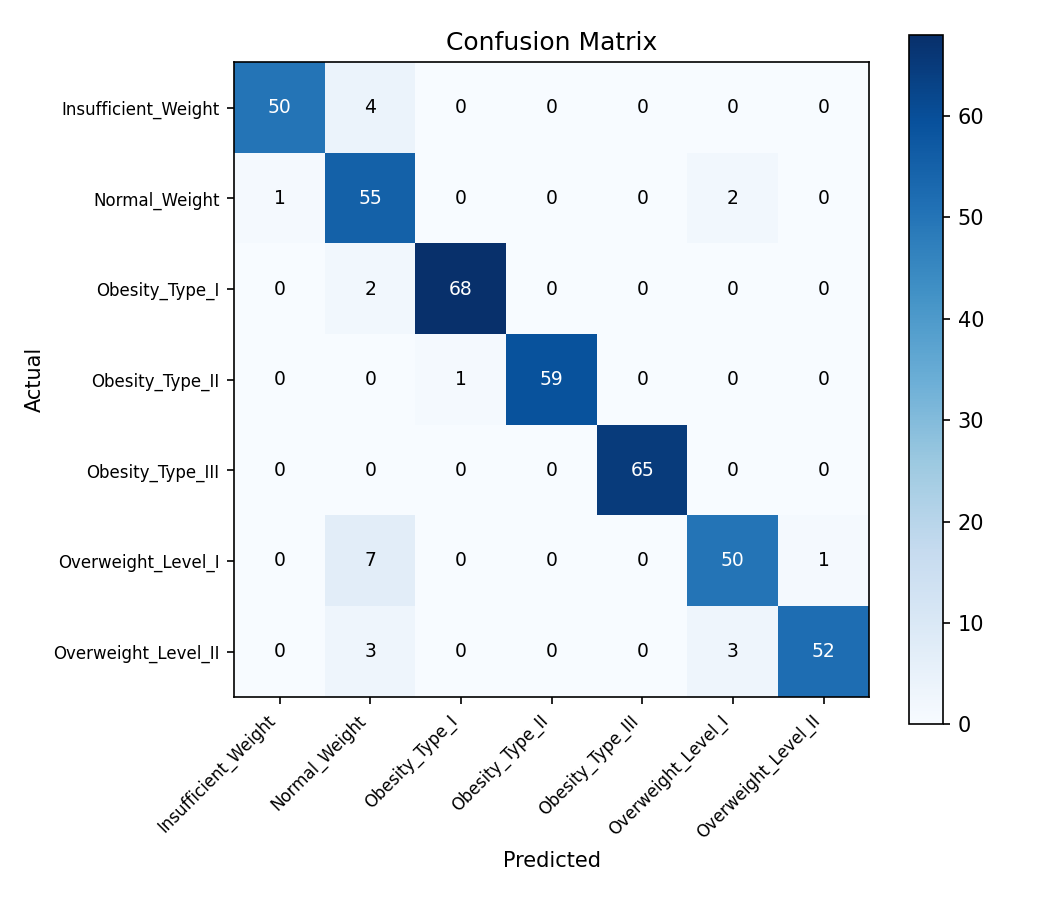
\includegraphics[width=\linewidth]{../results/02_benchmarks/obesity_level/confusion_matrix_random_forest.png}
    \caption{Random Forest}
  \end{subfigure}
  \hfill
  \begin{subfigure}{0.48\textwidth}
    \centering
    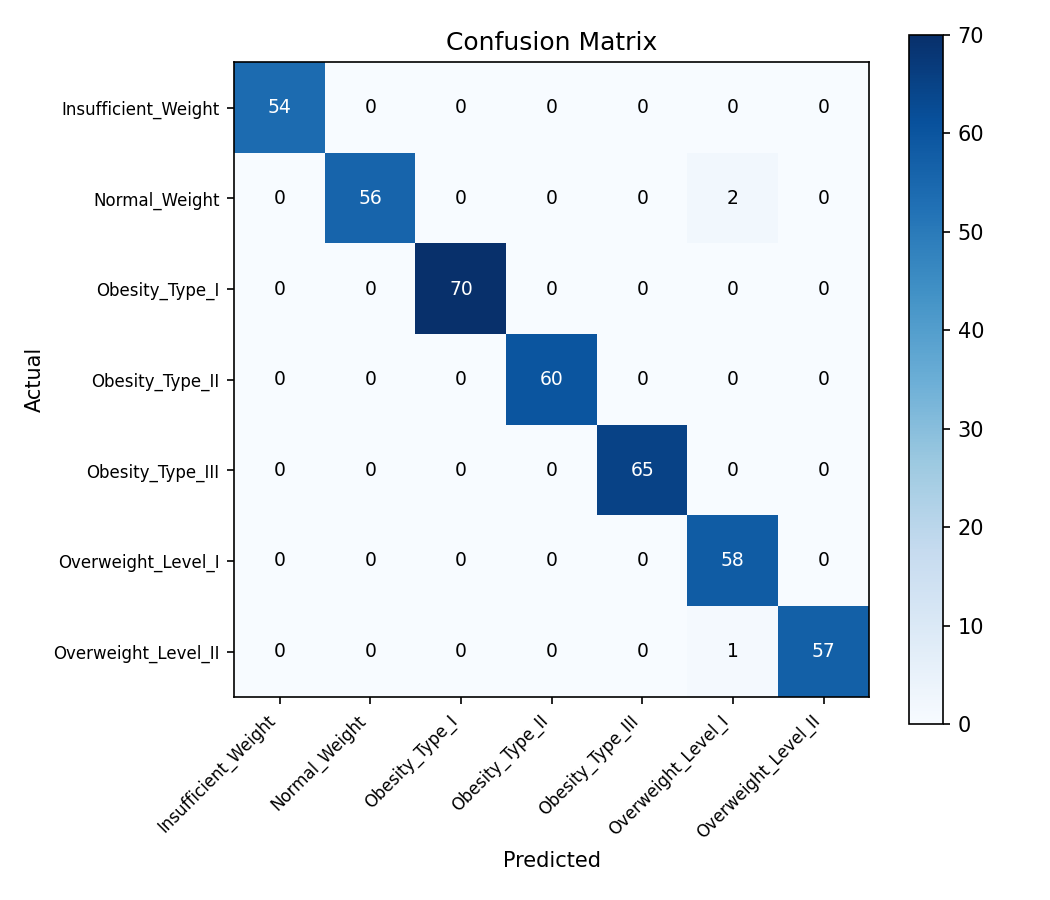
\includegraphics[width=\linewidth]{../results/02_benchmarks/obesity_level/confusion_matrix_tabpfn.png}
    \caption{TabPFN}
  \end{subfigure}

  \vspace{0.4cm}

  \begin{subfigure}{0.48\textwidth}
    \centering
    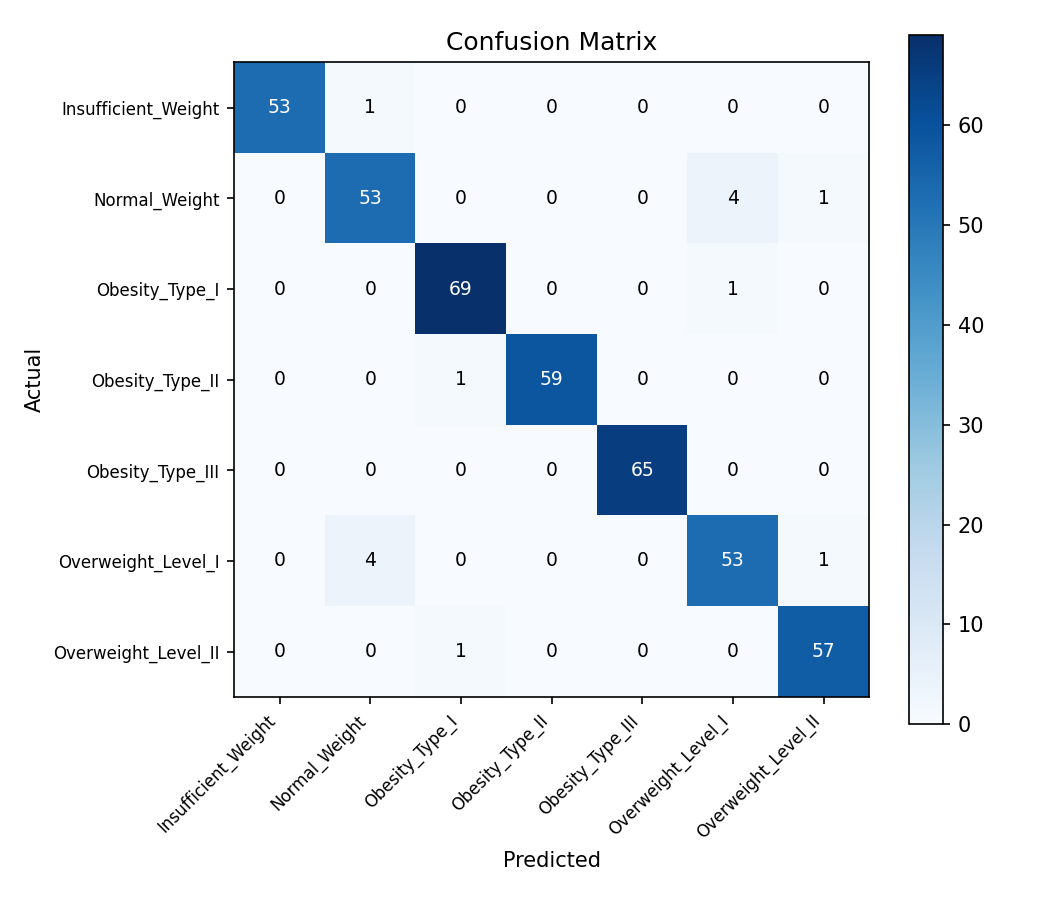
\includegraphics[width=\linewidth]{../results/02_benchmarks/obesity_level/confusion_matrix_xgboost.png}
    \caption{XGBoost}
  \end{subfigure}
  \hfill
  \begin{subfigure}{0.48\textwidth}
    \centering
    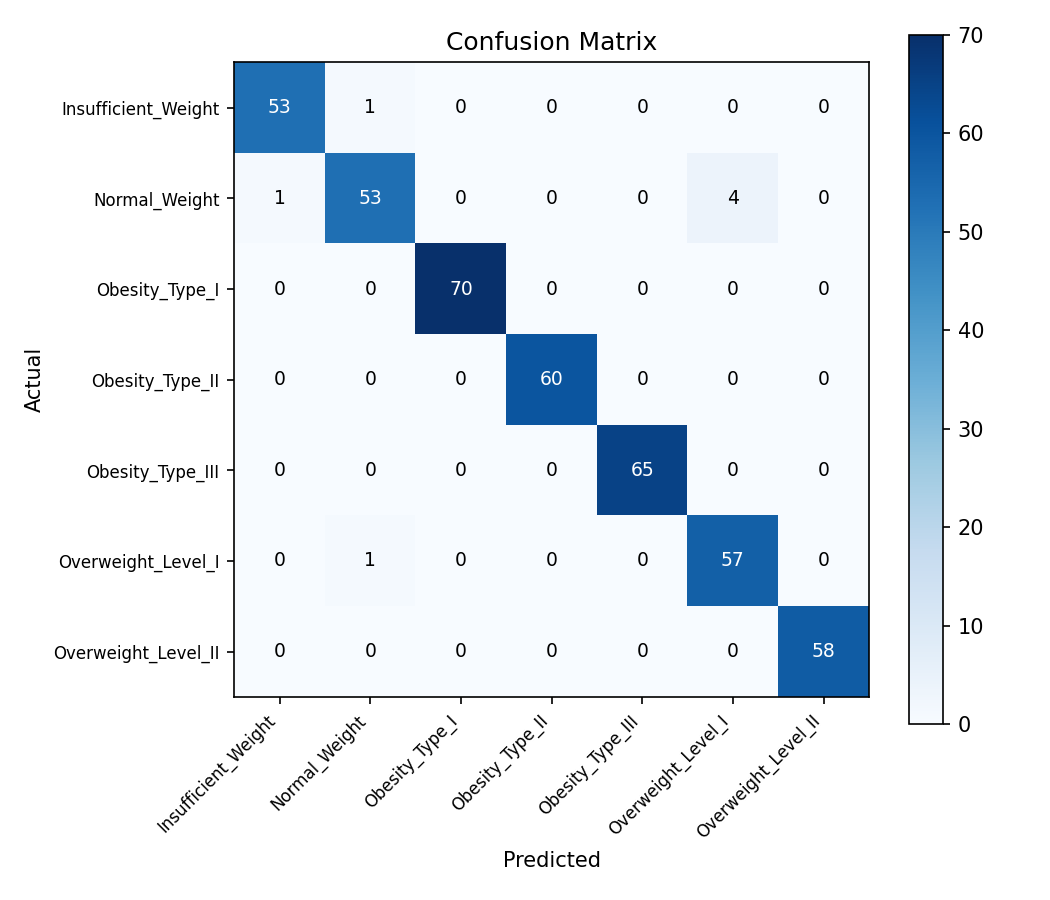
\includegraphics[width=\linewidth]{../results/02_benchmarks/obesity_level/confusion_matrix_xrfm.png}
    \caption{xRFM}
  \end{subfigure}

  \caption{Confusion matrices on the Obesity Level dataset.}
  \label{fig:cm-obesity}
\end{figure}

\subsection{Sleep Health}

\begin{figure}[H]
  \centering

  \begin{subfigure}{0.48\textwidth}
    \centering
    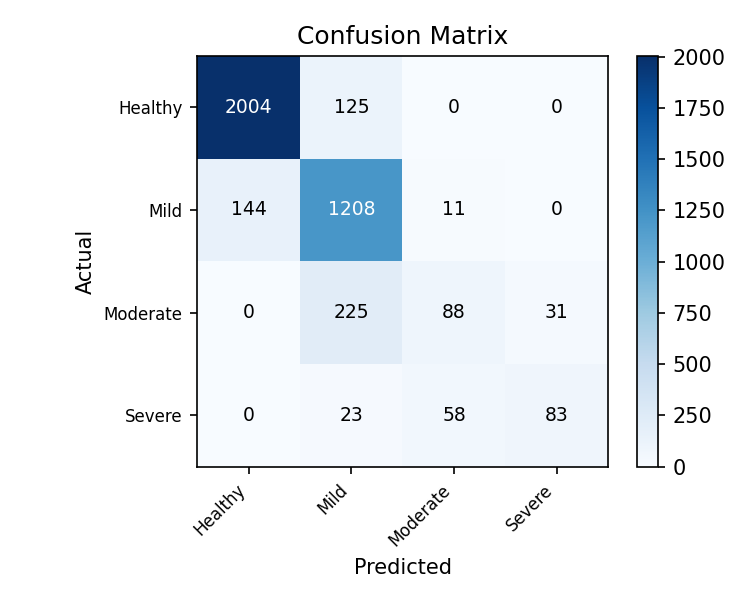
\includegraphics[width=\linewidth]{../results/02_benchmarks/sleep_health/confusion_matrix_random_forest.png}
    \caption{Random Forest}
  \end{subfigure}
  \hfill
  \begin{subfigure}{0.48\textwidth}
    \centering
    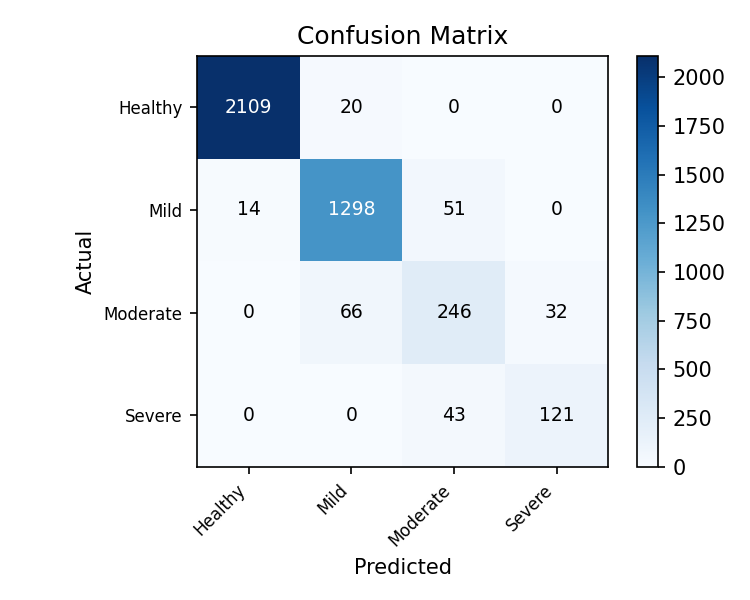
\includegraphics[width=\linewidth]{../results/02_benchmarks/sleep_health/confusion_matrix_tabpfn.png}
    \caption{TabPFN}
  \end{subfigure}

  \vspace{0.4cm}

  \begin{subfigure}{0.48\textwidth}
    \centering
    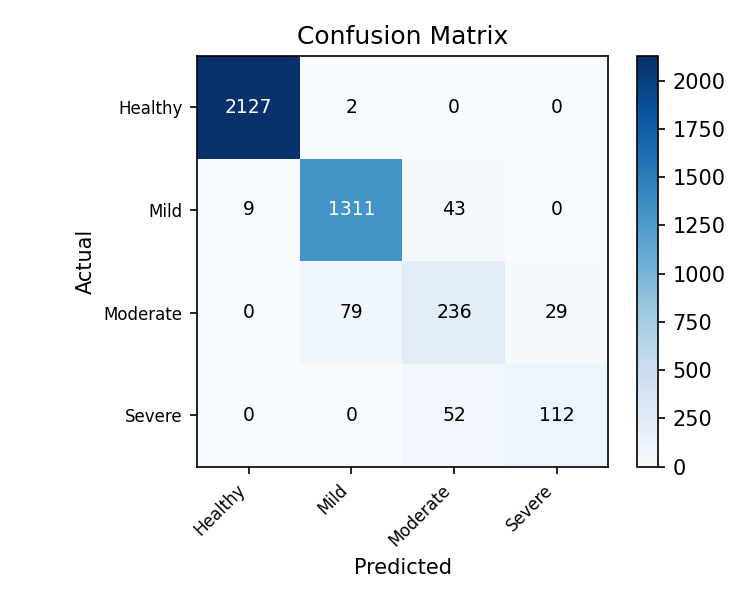
\includegraphics[width=\linewidth]{../results/02_benchmarks/sleep_health/confusion_matrix_xgboost.png}
    \caption{XGBoost}
  \end{subfigure}
  \hfill
  \begin{subfigure}{0.48\textwidth}
    \centering
    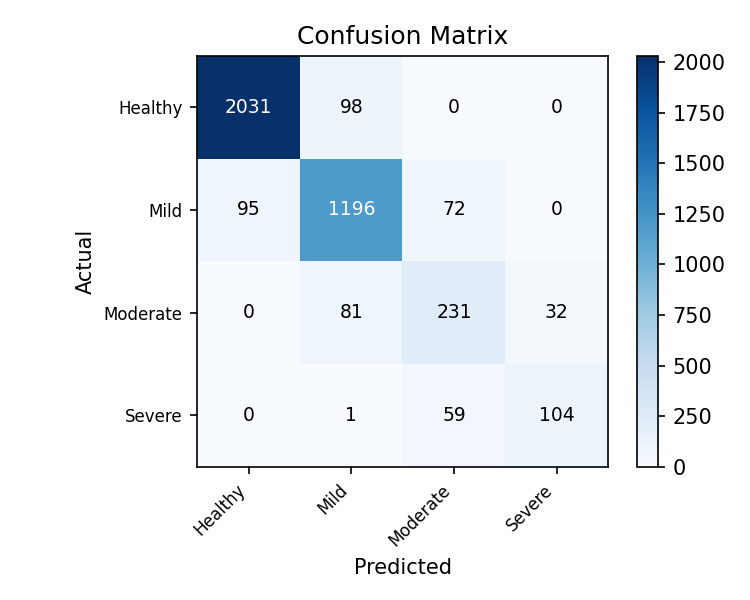
\includegraphics[width=\linewidth]{../results/02_benchmarks/sleep_health/confusion_matrix_xrfm.png}
    \caption{xRFM}
  \end{subfigure}

  \caption{Confusion matrices on the Sleep Health dataset.}
  \label{fig:cm-sleep-health}
\end{figure}
\clearpage
\section{AUC-ROC curves for classification datasets}

Figures~\ref{fig:roc-obesity} and~\ref{fig:roc-sleep} show the AUC-ROC curves for the two classification datasets. These curves illustrate the trade-off between true positive rate and false positive rate across different thresholds, complementing the AUC-ROC scores reported in the Results section.

\subsection{Obesity Level}

\begin{figure}[H]
  \centering

  \begin{subfigure}{0.48\textwidth}
    \centering
    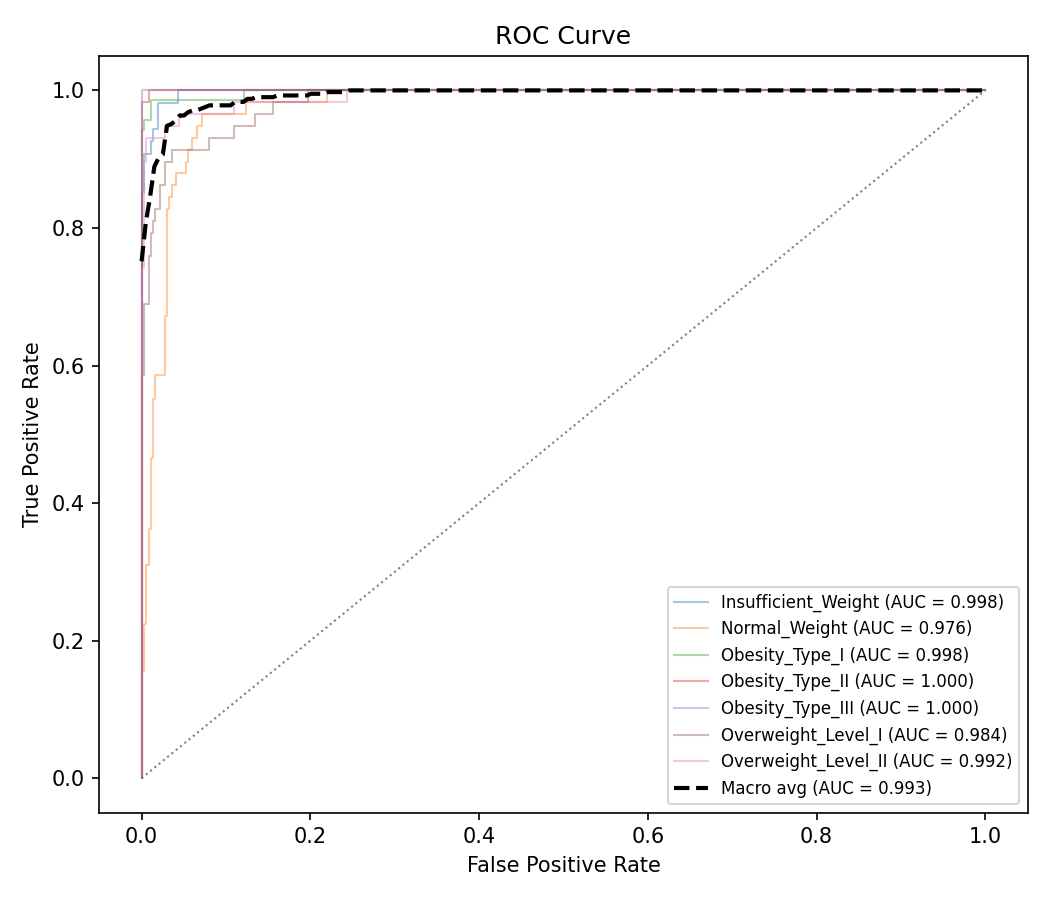
\includegraphics[width=\linewidth]{../results/02_benchmarks/obesity_level/roc_curve_random_forest.png}
    \caption{Random Forest}
  \end{subfigure}
  \hfill
  \begin{subfigure}{0.48\textwidth}
    \centering
    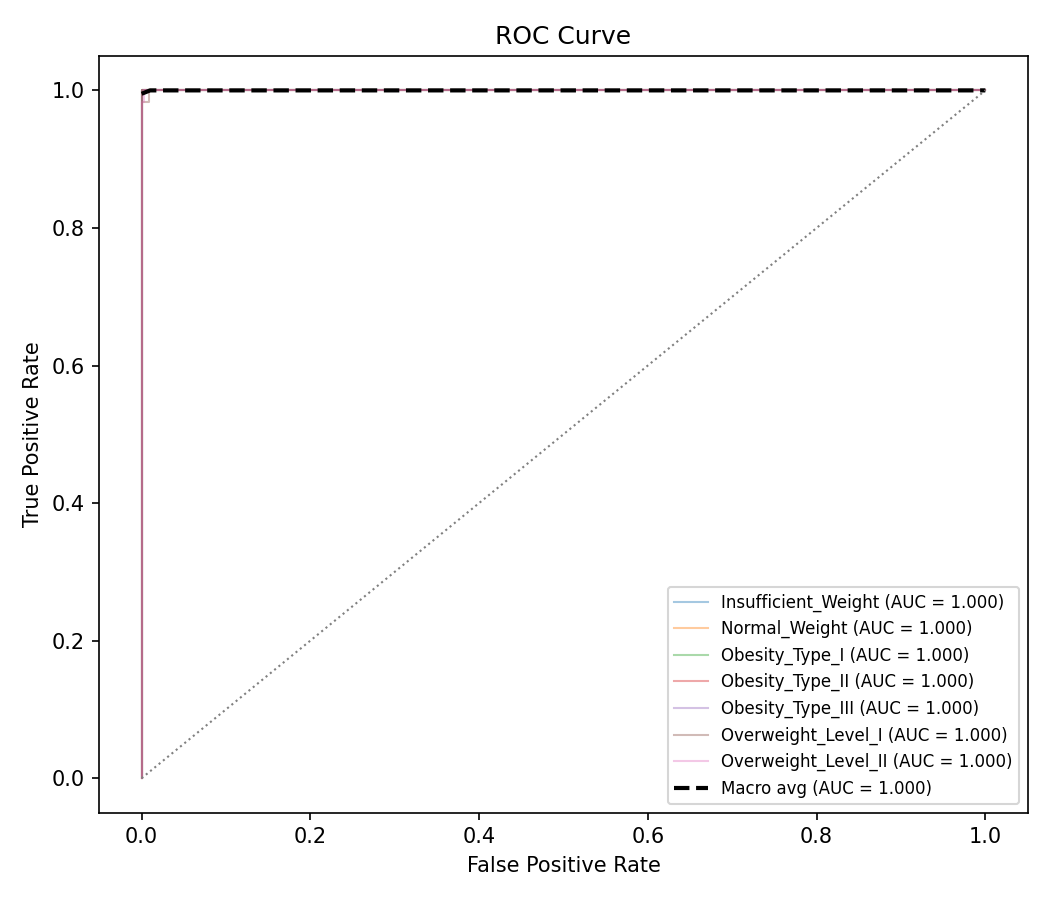
\includegraphics[width=\linewidth]{../results/02_benchmarks/obesity_level/roc_curve_tabpfn.png}
    \caption{TabPFN}
  \end{subfigure}

  \vspace{0.4cm}

  \begin{subfigure}{0.48\textwidth}
    \centering
    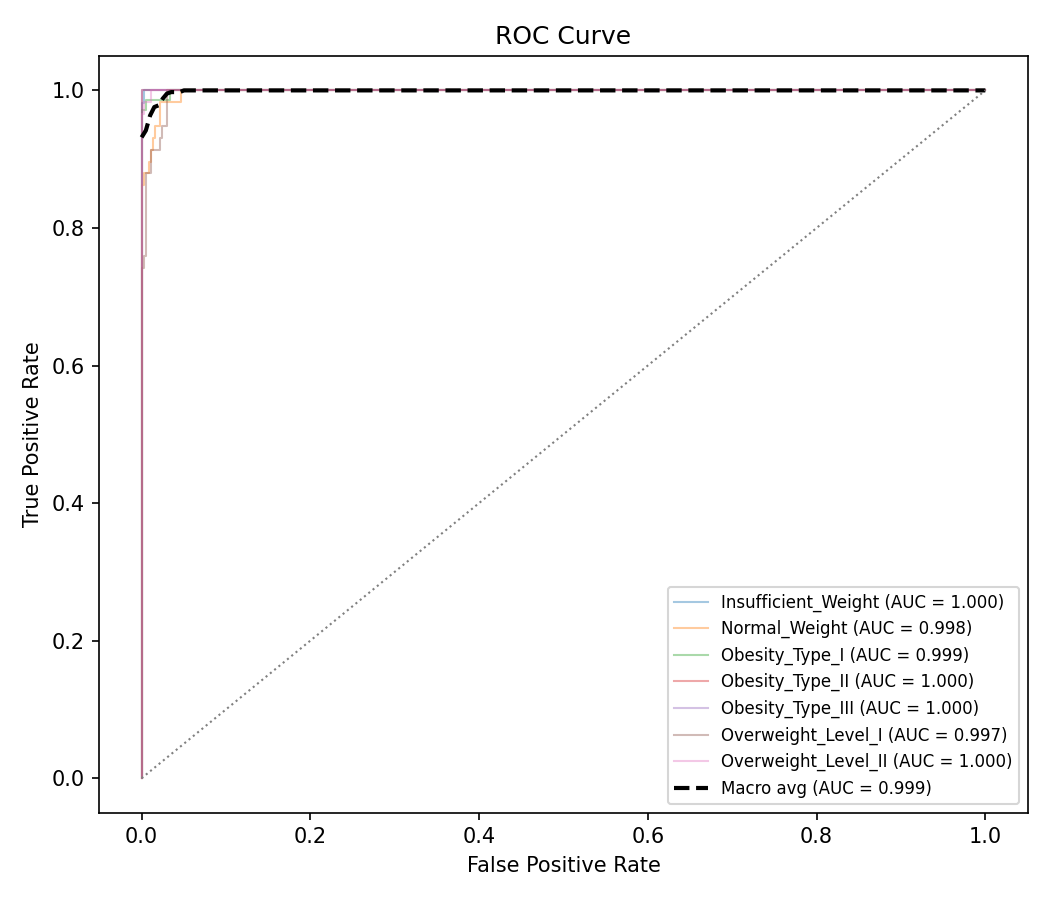
\includegraphics[width=\linewidth]{../results/02_benchmarks/obesity_level/roc_curve_xgboost.png}
    \caption{XGBoost}
  \end{subfigure}
  \hfill
  \begin{subfigure}{0.48\textwidth}
    \centering
    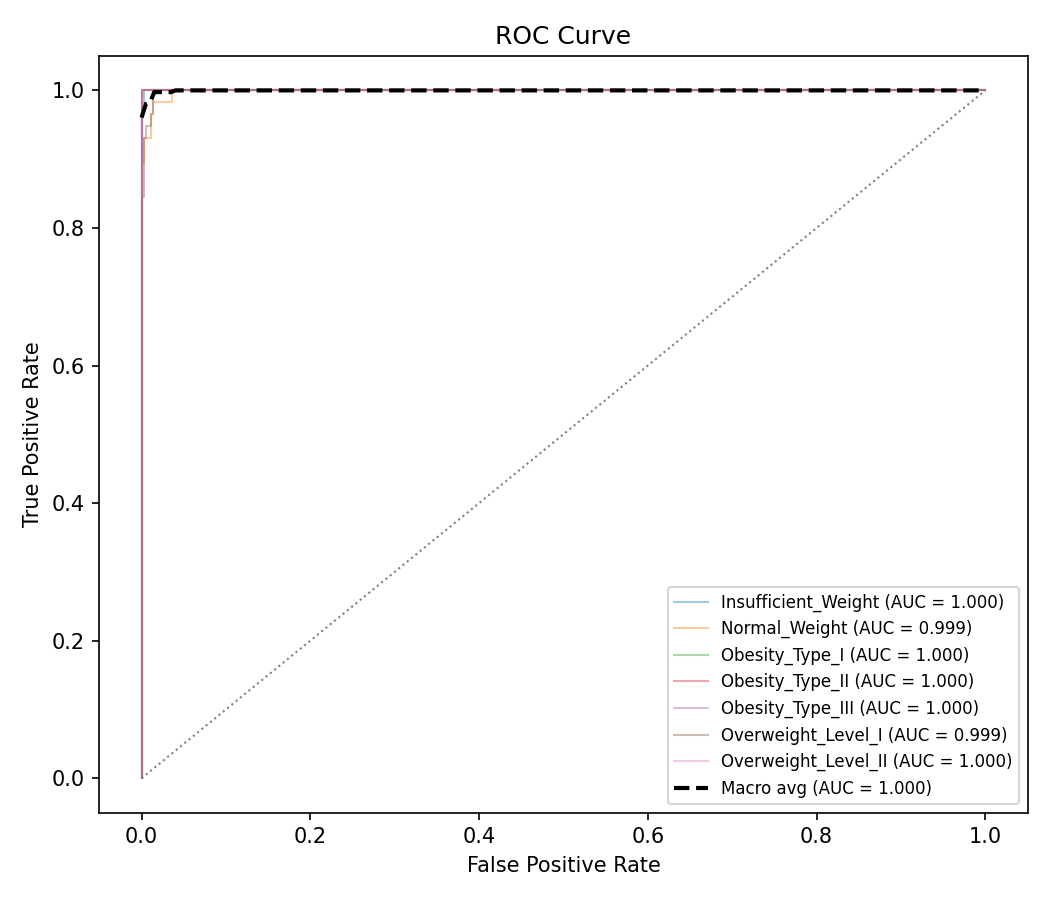
\includegraphics[width=\linewidth]{../results/02_benchmarks/obesity_level/roc_curve_xrfm.png}
    \caption{xRFM}
  \end{subfigure}

  \caption{AUC-ROC curves on the Obesity Level dataset.}
  \label{fig:roc-obesity}
\end{figure}

\subsection{Sleep Health}

\begin{figure}[H]
  \centering

  \begin{subfigure}{0.48\textwidth}
    \centering
    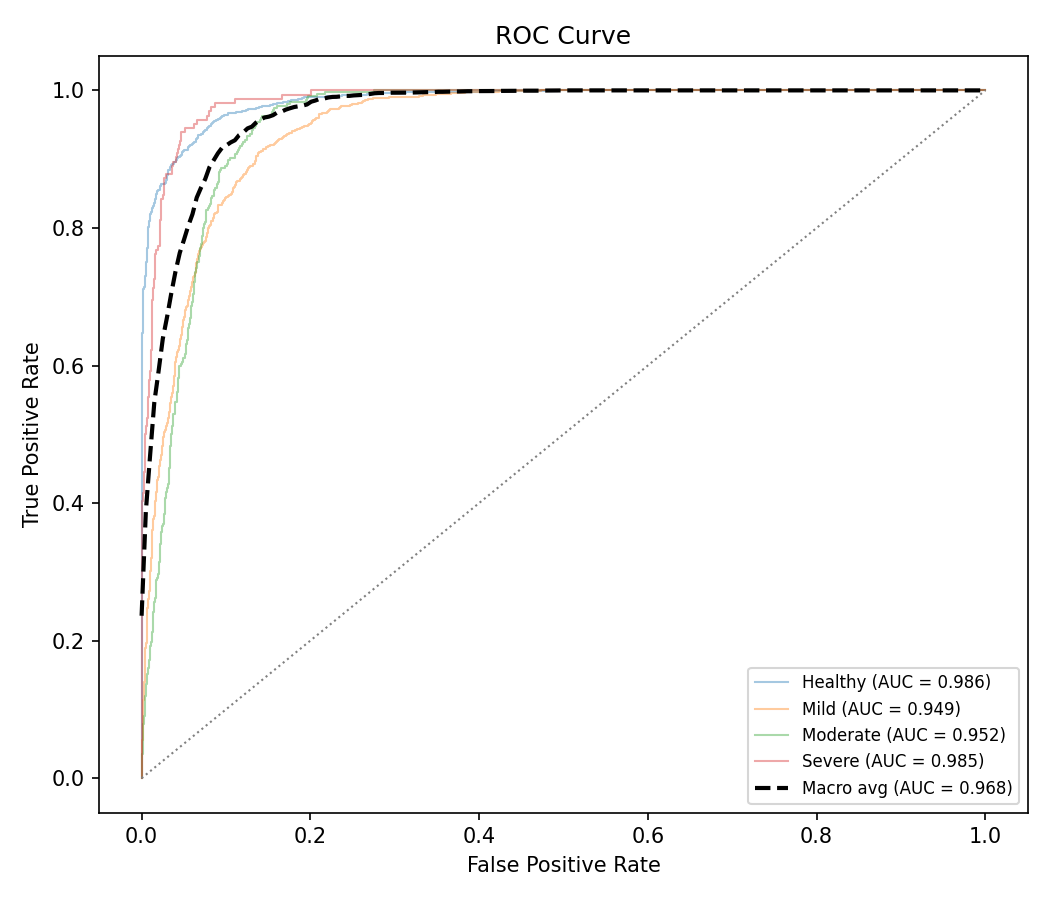
\includegraphics[width=\linewidth]{../results/02_benchmarks/sleep_health/roc_curve_random_forest.png}
    \caption{Random Forest}
  \end{subfigure}
  \hfill
  \begin{subfigure}{0.48\textwidth}
    \centering
    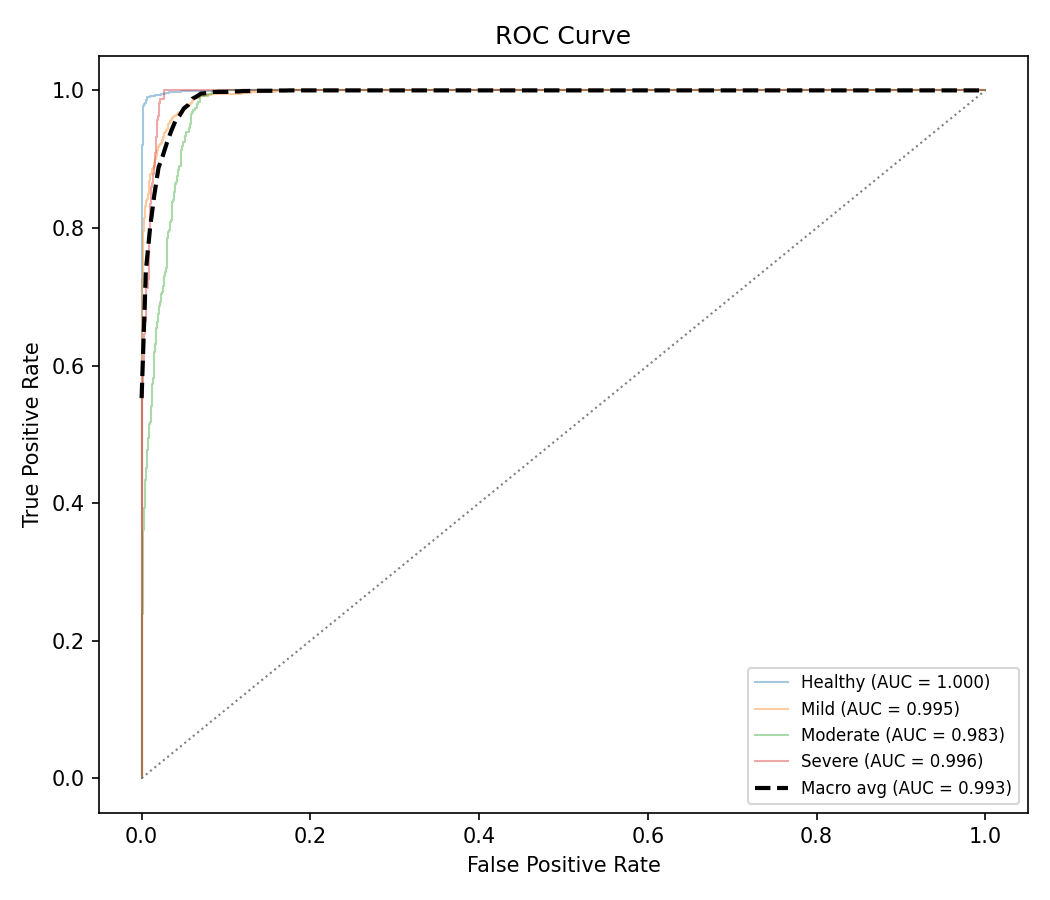
\includegraphics[width=\linewidth]{../results/02_benchmarks/sleep_health/roc_curve_tabpfn.png}
    \caption{TabPFN}
  \end{subfigure}

  \vspace{0.4cm}

  \begin{subfigure}{0.48\textwidth}
    \centering
    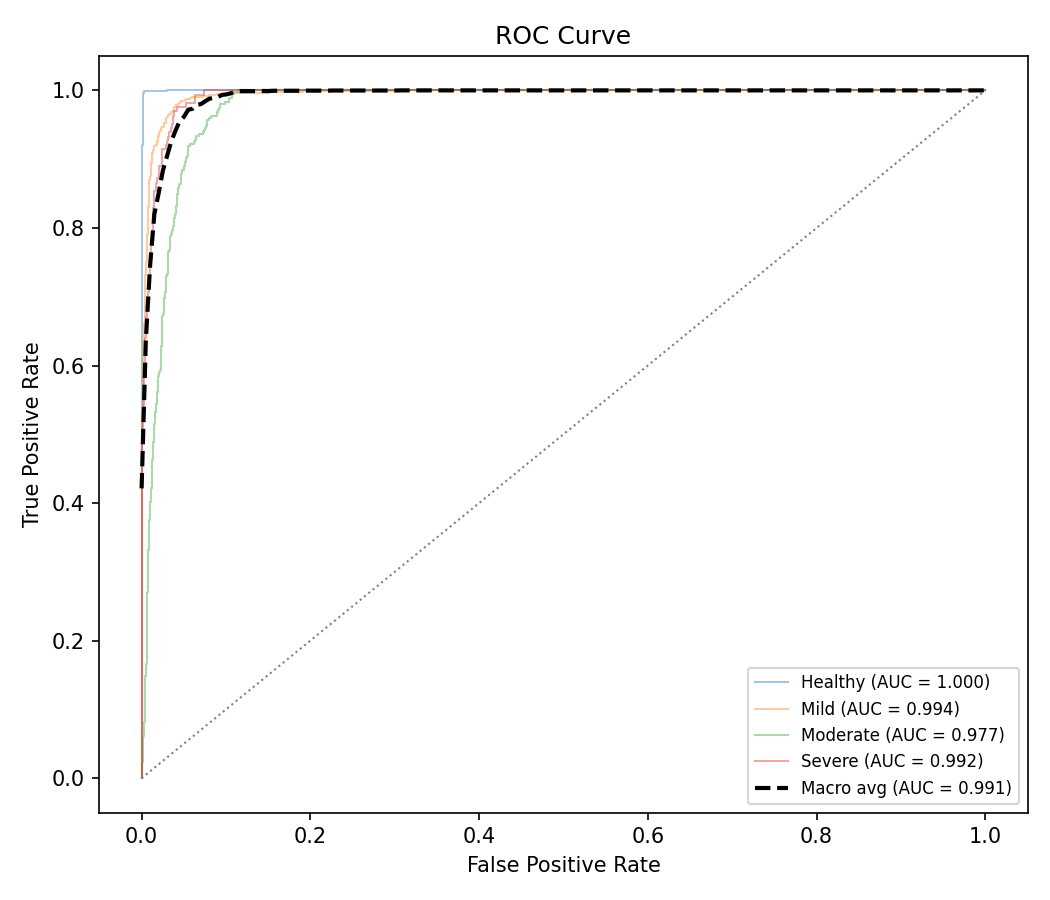
\includegraphics[width=\linewidth]{../results/02_benchmarks/sleep_health/roc_curve_xgboost.png}
    \caption{XGBoost}
  \end{subfigure}
  \hfill
  \begin{subfigure}{0.48\textwidth}
    \centering
    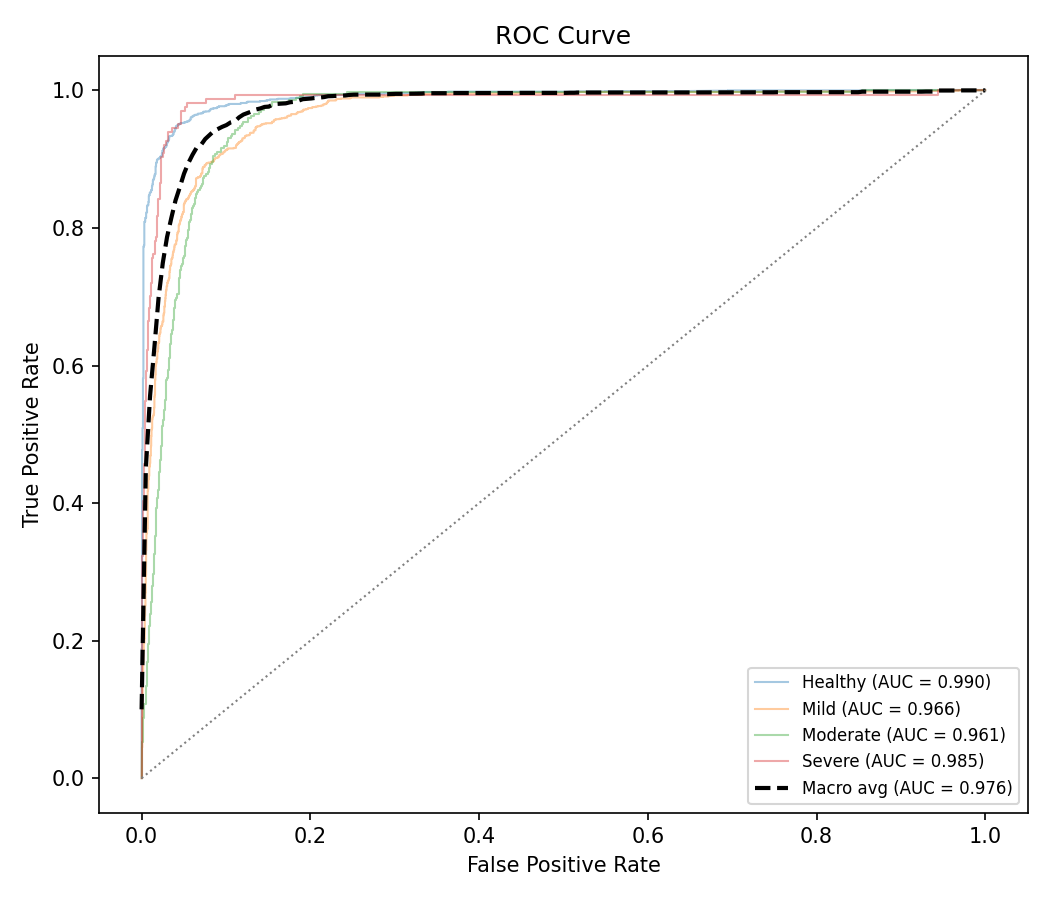
\includegraphics[width=\linewidth]{../results/02_benchmarks/sleep_health/roc_curve_xrfm.png}
    \caption{xRFM}
  \end{subfigure}

  \caption{AUC-ROC curves on the Sleep Health dataset.}
  \label{fig:roc-sleep}
\end{figure}
\clearpage
\section{Classification reports for classification datasets}

Accuracy (Acc.), precision (P), recall (R), and F1-score (F1) are reported. 

Table~\ref{tab:obesity_classification_report} summarises the classification report metrics for the Obesity Level dataset.

\subsection{Obesity Level}

\begin{table}[H]
  \centering
  \caption{Classification report summary on the Obesity Level dataset}
  \small
  \begin{tabular}{lccccccc}
    \toprule
    \textbf{Model} & \textbf{Acc.} 
    & \textbf{Macro P} & \textbf{Macro R} & \textbf{Macro F1}
    & \textbf{Weighted P} & \textbf{Weighted R} & \textbf{Weighted F1} \\
    \midrule
    Random Forest & 0.9433 & 0.9473 & 0.9411 & 0.9424 & 0.9491 & 0.9433 & 0.9445 \\
    TabPFN        & 0.9929 & 0.9930 & 0.9926 & 0.9927 & 0.9933 & 0.9929 & 0.9929 \\
    XGBoost       & 0.9669 & 0.9665 & 0.9658 & 0.9661 & 0.9670 & 0.9669 & 0.9669 \\
    xRFM          & 0.9835 & 0.9828 & 0.9826 & 0.9825 & 0.9837 & 0.9835 & 0.9834 \\
    \bottomrule
  \end{tabular}
  \label{tab:obesity_classification_report}
\end{table}


Table~\ref{tab:sleep_health_classification_report} summarises the classification report metrics for the Sleep Health dataset.
\subsection{Sleep Health}

\begin{table}[H]
  \centering
  \caption{Classification report summary on the Sleep Health dataset}
  \small
  \begin{tabular}{lccccccc}
    \toprule
    \textbf{Model} & \textbf{Acc.} 
    & \textbf{Macro P} & \textbf{Macro R} & \textbf{Macro F1}
    & \textbf{Weighted P} & \textbf{Weighted R} & \textbf{Weighted F1} \\
    \midrule
    Random Forest & 0.8458 & 0.7464 & 0.6474 & 0.6765 & 0.8350 & 0.8458 & 0.8331 \\
    TabPFN        & 0.9435 & 0.8614 & 0.8490 & 0.8549 & 0.9430 & 0.9435 & 0.9432 \\
    XGBoost       & 0.9465 & 0.8612 & 0.8325 & 0.8457 & 0.9448 & 0.9465 & 0.9454 \\
    xRFM          & 0.8905 & 0.8068 & 0.7843 & 0.7939 & 0.8909 & 0.8905 & 0.8904 \\
    \bottomrule
  \end{tabular}
  \label{tab:sleep_health_classification_report}
\end{table}

\end{document}
